\subsection{Particle MCMC for MJP inference}
\label{sec:pmcmc}
\subsubsection{A sequential Monte Carlo algorithm for MJPs inference}
We describe a sequential Monte Carlo algorithm for MJPs inference that underlies particle MCMC. 
Denote by $S_{[t_1', t_2']}$ the MJP trajectory from time $t_1'$ to time $t_2'$. 
Our target is to sample an MJP trajectory $S_{[0, t_{end}]}$ given $n$ noisy observations $X =(x_1, x_2, ... , x_n)$, at time $t_1^X, t_2^X, ..., t_n^X$. 
The initial value of the Markov jump process trajectory can be simulated from its initial distribution over states: $S(0) \sim \pi_0$. 
$S_{[t_i^X, t_{i + 1}^X]} $, its values over any interval $[t_i^X, t_{i+1}^X]$ can be simulated by Gillespie's algorithm as described in section~\ref{sec:???}. 
%Write the conditional distribution over states at time $t^X_{i+1}$ given value at time $t^X_i$ as $f_\theta(S(t^X_{i+1})|S(t^X_i))$, so that
%$S(t_{i + 1}^X) \sim f_\theta (\cdot | S(t_i^X))$.  
For the $i$th observation $x_i$ at time $t^X_i$, denote the likelihood for $S(t^X_i)$ as $P(x_i | S(t^X_i))$.
%Let $q_\theta^i$ be the important sampling proposal distribution. In our case, we set $q_\theta^i(\cdot| X_n, S_{[0, t^X_{n-1}]}) = f_\theta(S_{[t^X_{i-1},t_i]}| S_{[0, t^X_{i-1}]})$.% and $\mu_\theta$ as the prior Markov jump process density and 

%$S_{[0, t_{end}]}$ with rate matrix $A(\theta)$ can be characterized by 

%This procedure provides us at time $T$ with an approximation of the joint posterior density $p_%\theta(dS_{[0,T]}|X_{1:n})$ given by $$\hat{p_\theta}(dS_{[0,T]}|X_{1:n}) = \sum_{k =1}^N W_n^k %\delta_{S^k[0:T]}(dS_{[0,T]})$$\\
%In addition, the estimate of the marginal likelihood $p_\theta(y_{1:n})$ is given by 
%$$\hat{p}_\theta(X_{1:n}) = \hat{p}_\theta(X_1) \prod_{i = 2}^n \hat{p}_\theta(X_i | X_{i -1}) $$\\
%where$$\hat{p}_\theta(y_i | y_{i -1}) = \frac{1}{N} \sum_{k = 1}^ N w_n(S_{[0, t_i]}) $$
%is an estimate computed at time $i$ of 
%$$p_\theta(X_i | X_{i -1}) = \int w_n(S_{[0,t_i]}) q_\theta(S_{[t_{i-1}, t_i]}| X_i, S_{[0, t_{i-1}]}) p_%\theta(S_{[0, t_{i-1}]}|X_{1: i-1}) dS_{[0,t_i]}.$$

\begin{algorithm}[H]
  \caption{The SMC sampler for MJP trajectories}
   \label{alg:SMC}
  \begin{tabular}{l l}
   \textbf{Input:  } & \text{Prior $\pi_0$, $n$ observations $X$}, 
                       \text{Number of particles $N$}, rate-matrix $A$.\\
                     %& MJP rate-matrix $A$\\
   \textbf{Output:  }& \text{New MJP trajectory $S' (t) = (s'_0, S', T')$}.\\
   \hline
   \end{tabular}
   \begin{algorithmic}[1]
\State Define $t^X_0 = 0$ and $t^X_{n+1} = t_{end}$. %Define $J^k_0$
\State 
Sample initial states for N particles $S^k(0)$ from $\pi_0$, $k = 1,...,N$. 
\State For $i = 1, ..., n+1$:\\
\noindent \noindent (a) For $k = 1,2,...,N$,\\ update particle $k$ from $[0,t^X_{i-1}]$ to $[0,t^X_i]$ by forward simulating $S_{[t^X_{i -1},t^X_i]}^k|S^k(t^X_{i-1})$ via Gillespie's algorithm. \\
%\noindent \noindent (b) Sample $S_{[t^X_{i -1},t^X_i]}^k \sim q_\theta^i(\cdot| X_i, S_{[0, t_{i-1}^X]}^{J_{i-1}^k})$, $k = 1,2,...,N$;\\
%\boqian{Simulate $S_{[t^X_{i -1},t^X_i]}^k|S^{J_{i-1}^k}_{t^X_{i-1}}$ via Gillespie's algorithm, for $k = 1,2,...,N$;}
\noindent \noindent (d) Calculate the weights $w^k_i = P(x_i|S^k(t^X_i))$
and normalize 
$W^k_i = \frac{w^k_i}{\sum_{k = 1}^N w^k_i}.$ \\
%
%
\noindent \noindent (a) Sample $J_{i}^k \sim \text{Multi}(\cdot| (W^1_{i},\dotsc,W^N_{i}))$ , $k = 1,2,...,N$;\\
\noindent \noindent (c) Set $S_{[0, t^X_i]}^k := S_{[0,t^X_i]}^{J^k_i}$.
\end{algorithmic}
\end{algorithm}

%At time $t_{end}$ uniformly pick a particle. It

The SMC algorithm gives us an estimate of the marginal likelihood $P_\theta(X_{1:n})$.
$$ \hat{P}_{\theta} = \hat{P}_{\theta}(X_1) \prod_{i = 2}^n \hat{P}_{\theta}(X_i| X_{1: i- 1}) = ????;$$
%where $\hat{P}_{\theta}(X_i| X_{1: i- 1}) = \sum_{k = 1} ^ N w_i(S_{[t_0^X, t_I^X]}^k).$


\subsubsection{Particle MCMC algorithm for MJPs inference}

\begin{algorithm}[H]
  \caption{The particle marginal MH sampler for MJP trajectories}
   \label{alg:SMC}
  \begin{tabular}{l l}
   \textbf{Input:  } & \text{Prior $\pi_0$, observations $X$}, 
                       \text{Number of particles $N$}, rate-matrix $A(\theta)$,\\
                     & $P(\theta)$ prior of $\theta$, proposal density $q(\cdot|\cdot)$. \\
   \textbf{Output:  }& \text{New MJP trajectory $S' (t) = (s'_0, S', T')$}.\\
   \hline
   \end{tabular}
   \begin{algorithmic}[1]
\State At time $i = 0$:\\
\noindent Set $\theta_0$ arbitrarily;
\noindent Run the SMC algorithm above targeting $P_{\theta_0}(S_{[0, T]} | X_{1:n})$ to sample $S_{[0, T]}(0)$ from $\hat{P}_{\theta_0}(\cdot | X_{1:n})$ and let $\hat{P}_{\theta_0}(X_{1:n})$ denote the estimate of the marginal likelihood.
\State At time $i \geq 1:$\\
\noindent \noindent (a) Sample $\theta^*$ from a proposal distribution $q(\cdot | \theta_{i - 1})$;
\noindent \noindent (b) Run the SMC algorithm above targeting $P_{\theta^*}(S_{[0, T]} | X_{1:n})$ to sample $S_{[0, T]}^*$ from $\hat{P}_{\theta^*}(\cdot | X_{1:n})$ and let $\hat{P}_{\theta^*}(X_{1:n})$ denote the estimate of the marginal likelihood.
\noindent Accept $\theta^*, S_{[0, T]}^*$ with probability $$ \mathtt{acc} = 1 \wedge \frac{\hat{P}_{\theta^*}(X_{1:n}) p(\theta^*)}{\hat{P}_{\theta_{i - 1}}(X_{1:n}) p(\theta_{i  - 1})} \frac{q(\theta_{i - 1} | \theta^*)}{q(\theta^* | \theta_{i - 1})}.$$

\end{algorithmic}
\end{algorithm}


\subsection{Algorithm sketch}
\setlength{\unitlength}{0.8cm}
  \begin{figure}[H]
  \centering
  \begin{minipage}[!hp]{0.45\linewidth}
  \centering
    \includegraphics [width=0.70\textwidth, angle=0]{figs/plotn0.pdf}
      \end{minipage}
  \begin{minipage}[!hp]{0.45\linewidth}
  \centering
    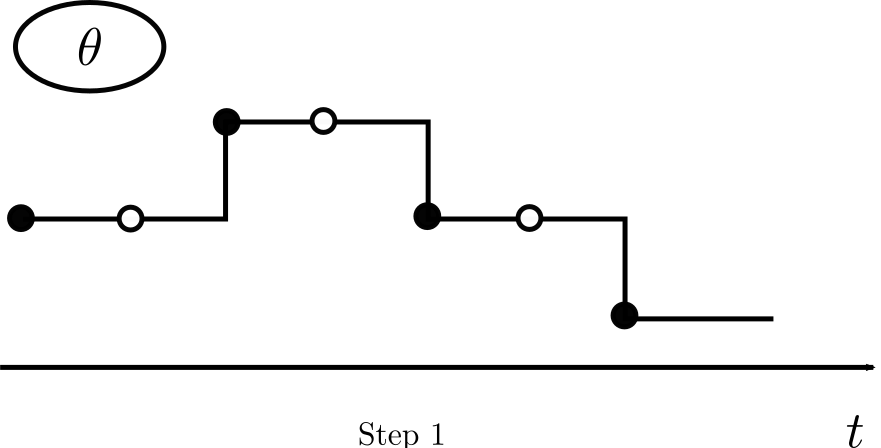
\includegraphics [width=0.70\textwidth, angle=0]{figs/plotn1.pdf}
    \vspace{-0 in}
  \end{minipage}
  \begin{minipage}[!hp]{0.45\linewidth}
  \centering
    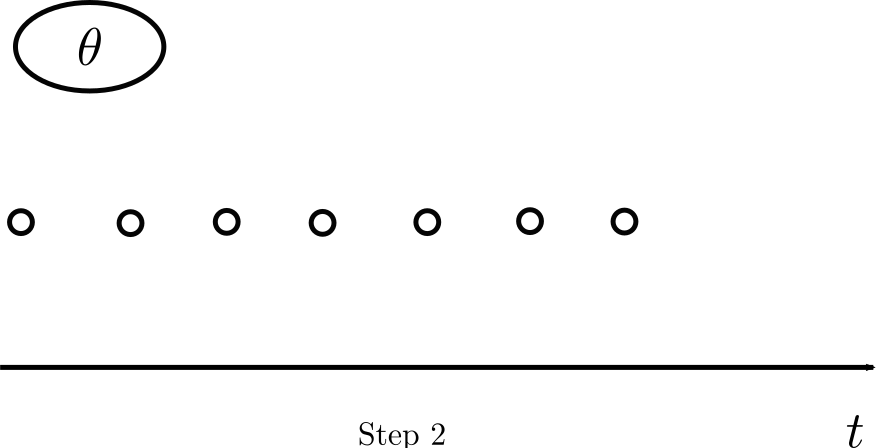
\includegraphics [width=0.70\textwidth, angle=0]{figs/plotn2.pdf}
    \vspace{-0 in}
  \end{minipage}
  \begin{minipage}[!hp]{0.45\linewidth}
  \centering
    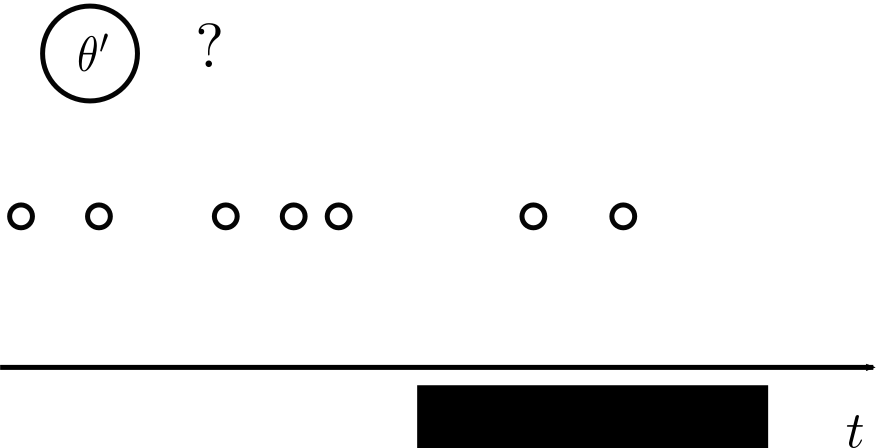
\includegraphics [width=0.70\textwidth, angle=0]{figs/plotn3.pdf}
    \vspace{-0 in}
  \end{minipage}
  \begin{minipage}[!hp]{0.45\linewidth}
  \centering
    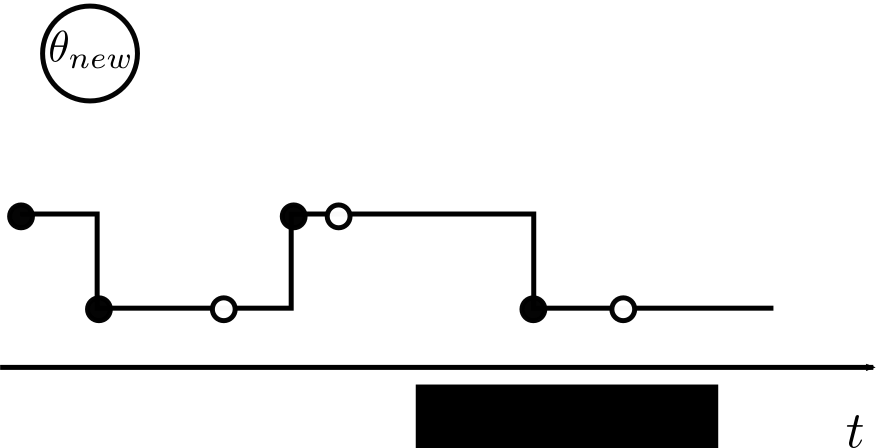
\includegraphics [width=0.70\textwidth, angle=0]{figs/plotn4.pdf}
    \vspace{-0 in}
  \end{minipage}
  \begin{minipage}[!hp]{0.45\linewidth}
  \centering
    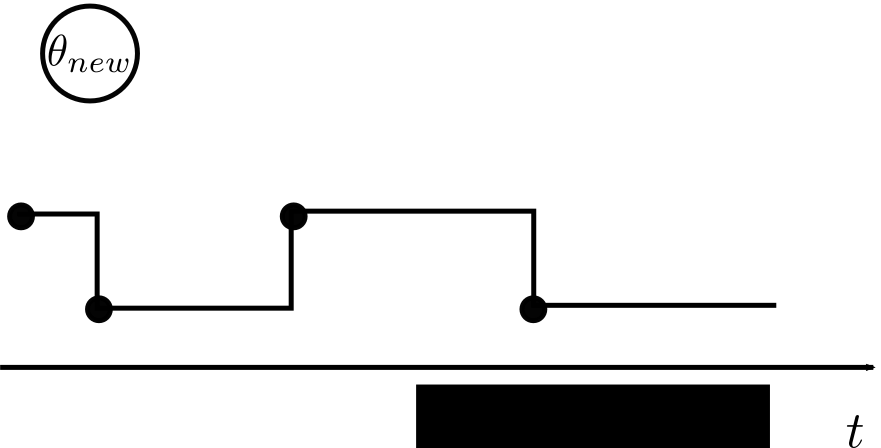
\includegraphics [width=0.70\textwidth, angle=0]{figs/plotn5.pdf}
    \vspace{-0 in}
  \end{minipage}
  \caption{\Naive\ MH-algorithm: Step 0 to 2: sample thinned events
  and discard state information to get a random grid. Step 3: 
propose a new parameter $\theta'$, and accept or reject by making
a forward pass on the grid. Steps 4 to 5: make a backward pass using
the accepted parameter and discard self-transitions to produce a new
trajectory.}
   \label{fig:naive_mh}
  \end{figure}

\subsection{Additional results}
In the following, we evaluate Python implementations of a number of algorithms, focusing our contribution, the symmetrized MH algorithm (algorithm~\ref{alg:MH_improved}), and as well as the \naive\ MH algorithm (algorithm~\ref{alg:MH_naive}).
%, which we plot \boqian{as yellow twodashed  lines}), 
%, plotted \sout{as dashed red lines}\boqian{as solid blue lines}
We evaluate different variants of these algorithms, corresponding to different uniformizing Poisson rates. % (i.e.\ different choices of $\kappa$, see section~\ref{sec:comments}). 
For \naive\ MH, we set $\Omega(\theta) = \kappa \max_s A_s(\theta) $ with $\kappa$  equal to $1.5, 2$ and $3$ (here $\kappa$ must be greater than $1$), 
%represented in our plots with circles, \sout{triangles} \boqian{square} and \sout{square} \boqian{triangles} symbols. 
while for symmetrized MH, where the uniformizing rate depends on both the current and proposed parameters, we consider the settings:
 $\Omega(\theta, \vartheta) = \kappa (\max A(\theta) + \max A(\vartheta))$ 
 ($\kappa = 1$ and $1.5$), and 
 %, plotted with \sout{triangles} \boqian{square} and \sout{square} \boqian{triangles}), and 
$\Omega(\theta, \vartheta) = 1.5 \max(\max A(\theta), \max A(\vartheta))$.
%($\kappa=1.5$, plotted with {circles}).  
We evaluate two other baselines: Gibbs sampling (Algorithm~\ref{alg:MJP_gibbs}), %plotted \sout{in blue} \boqian{as red long dashed lines} ), 
and particle MCMC~\citep[][see also section~\ref{sec:pmcmc} in the appendix]{Andrieu10}. 
%plotted \sout{in black} \boqian{as black dashed lines}. 
Gibbs sampling involves a uniformization step to update the MJP trajectory (step 1 in algorithm~\ref{alg:MJP_gibbs}), for which we use $\Omega(\theta,\vartheta) = \kappa \max_s A_s(\theta)$ for $\kappa=1.5,2,3$. 
%plotted with circles, \sout{triangles} \boqian{square} and \sout{square} \boqian{triangles}.  
Unless specified, our results were obtained from $100$ independent MCMC runs, each of $10000$ iterations.
We found particle MCMC to be more computationally intensive, and limited each run to $3000$ iterations, the number of particles being $5, 10$ and $20$.
For each run of each MCMC algorithm, we calculated the effective sample size (ESS) of the posterior samples of the MJP parameters using the R package \texttt{rcoda}~\citep{Rcoda2006}. 
This estimates the number of independent samples returned by the MCMC algorithm, and dividing this by the runtime of a simulation gives the ESS per unit time (ESS/sec). 
We used this to compare different samplers and different parameter settings. In the following we present the additional results.

  \begin{figure}[H]
  \centering
  \begin{minipage}[h!]{0.99\linewidth}
  \centering
    \includegraphics [width=0.24\textwidth, angle=0]{figs/new_whole_exp_figs/exp_alpha_dim3.pdf}
    \includegraphics [width=0.24\textwidth, angle=0]{figs/new_whole_exp_figs/exp_beta_dim3.pdf}
    \includegraphics [width=0.24\textwidth, angle=0]{figs/new_whole_exp_figs/exp_alpha_dim10.pdf}
    \includegraphics [width=0.24\textwidth, angle=0]{figs/new_whole_exp_figs/exp_beta_dim10.pdf}
  \end{minipage}

  \begin{minipage}[h!]{0.49\linewidth}
  \centering
    \includegraphics [width=0.49\textwidth, angle=0]{figs/new_whole_exp_figs/exp_alpha_dim5.pdf}
    \includegraphics [width=0.49\textwidth, angle=0]{figs/new_whole_exp_figs/exp_beta_dim5.pdf}
  \end{minipage}
  \begin{minipage}[!hp]{0.49\linewidth}
    \caption{ESS/sec for the synthetic model, The top left two panels are $\alpha$ and $\beta$ for 3 states, the bottom two, for 5 states, and the right two, for 10 states. Blue, yellow, red and black are the symmetrized MH, \naive\ MH, Gibbs and particle MCMC algorithm.  Squares, circles and trianges correspond to $\Omega(\theta,\vartheta)$ set to $(\max_s A_s(\theta) + \max_s A_s(\vartheta))$, $\max(\max_s A_s(\theta), \max_s A_s(\vartheta))$ and  $1.5(\max_s A_s(\theta) + \max_s A_s(\vartheta))$. And for PMCMC, they correspond to 10 particles, 5 particles and 15 particles.}
     \label{fig:ESS_EXP}
  \end{minipage}
  \end{figure}


  \begin{figure}[H]
%    \vspace{-.2in}
  \centering
  \begin{minipage}[!hp]{0.99\linewidth}
    \includegraphics [width=0.24\textwidth, angle=0]{figs/acc/EXP_D3alpha_k2.pdf}
    \includegraphics [width=0.24\textwidth, angle=0]{figs/acc/EXP_D5alpha_k2.pdf}
    \includegraphics [width=0.24\textwidth, angle=0]{figs/EXP_ks/exp_traceoMH_7_05_3_.pdf}
    \includegraphics [width=0.24\textwidth, angle=0]{figs/EXP_ks/exp_omhacf_7_05_3_.pdf}
  \end{minipage}
%  \begin{minipage}[!hp]{0.49\linewidth}
    \caption{Acceptance Rate for $\alpha$ in the synthetic model (Left two), the first being dimension 3, and the second,dimension 5. Blue square and yellow triangle curves are the symmetrized MH, and \naive\ MH  algorithm. The multiplicative factor is $2$. Trace and autocorrelation plots for \naive\ MH  (right two panels) for the synthetic model with $3$ states.}
     \label{fig:ACC_EXP}
%  \end{minipage}
  \end{figure}
%  \begin{figure}[H]

%  \centering

%  \begin{minipage}[!hp]{0.99\linewidth}
%  	\centering
 %   \includegraphics [width=0.3\textwidth, angle=0]{figs/acc/JCalpha_k2.pdf}
%	\hspace{.5in}
  %  \includegraphics [width=0.3\textwidth, angle=0]{figs/JC_ks/jc_hist_44_05_3_.pdf}
  %\end{minipage}
%  \begin{minipage}[!hp]{0.99\linewidth}
   % \caption{The left represents the acceptance rate for $\alpha$ in the JC69 model.  Blue and yellow curves represent symmetrized MH,and \naive\ MH  algorithm. The multiplicative factor is $2$.The right is histogram for the posterior samples($\alpha$) of the JC69 model, the red and blue curves are the Gibbs and symmetrized MH. The p value of the two sample-Kolmogorov Smirnov test is $ 0.97$.  }
  %   \label{fig:ACC_JC}
%  \end{minipage}
  %\end{figure}
  
  \begin{figure}[H]
%    \vspace{-.2in}
  \centering
%  \begin{minipage}[!hp]{0.99\linewidth}
 % \centering
  \begin{minipage}[!hp]{0.99\linewidth}
    \includegraphics [width=0.24\textwidth, angle=0]{figs/Q_ks/q_traceGBS_20_03_3_.pdf}
    \includegraphics [width=0.24\textwidth, angle=0]{figs/Q_ks/q_traceMH_20_03_3_.pdf}
    \includegraphics [width=0.24\textwidth, angle=0]{figs/Q_ks/q_gbsacf_20_03_3_.pdf}
    \includegraphics [width=0.24\textwidth, angle=0]{figs/Q_ks/q_mhacf_20_03_3_.pdf}
  \end{minipage}
  
%  \end{minipage}
%  \begin{minipage}[!hp]{0.99\linewidth}
%    \caption{The left is histogram for the posterior samples($\alpha$) of the immigration model with dimension 3, the red and blue curves are the Gibbs and symmetrized MH. The p value of the two sample-Kolmogorov Smirnov test is $ 0.978$. The middle and the right are trace plots for the posterior samples of the immigration model with dimension 3, the middle is for Gibbs and the right is for symmetrized MH}
\caption{Trace and autocorrelation plots for Gibbs (left two panels) and symmetrized MH (right two panels). All plots are for the immigration model with $3$ states.}
     \label{fig:TRACE_Q}
%  \end{minipage}
  \end{figure}
  
  \begin{figure}[H]
%    \vspace{-.2in}
  \centering
%  \begin{minipage}[!hp]{0.99\linewidth}
 % \centering
  \begin{minipage}[!hp]{0.99\linewidth}
    \includegraphics [width=0.24\textwidth, angle=0]{figs/QC_ks/qc_traceGBS_4_03_10_.pdf}
    \includegraphics [width=0.24\textwidth, angle=0]{figs/QC_ks/qc_traceMH_4_03_10_.pdf}
    \includegraphics [width=0.24\textwidth, angle=0]{figs/QC_ks/qc_gbsacf_4_03_10_.pdf}
    \includegraphics [width=0.24\textwidth, angle=0]{figs/QC_ks/qc_mhacf_4_03_10_.pdf}
  \end{minipage}

%  \end{minipage}
%  \begin{minipage}[!hp]{0.99\linewidth}
%    \caption{The left is histogram for the posterior samples($\alpha$) of the time-inhomogeneous immigration model with dimension 10, the red and blue curves are the Gibbs and symmetrized MH. The p value of the two sample-Kolmogorov Smirnov test is $ 0.7212$. The middle and the right are trace plots for the posterior samples of the time-inhomogeneous immigration model with dimension 10, the middle is for Gibbs and the right is for symmetrized MH}
\caption{Trace and autocorrelation plots for Gibbs (left two panels) and symmetrized MH (right two panels). All plots are for the time-inhomogeneous immigration model with $10$ states.}
 
     \label{fig:TRACE_CQ}
%  \end{minipage}
  \end{figure}


  \begin{figure}[H]
  \centering
  \begin{minipage}[h!]{0.99\linewidth}
  \centering
    \includegraphics [width=0.24\textwidth, angle=0]{figs/new_whole_exp_figs/q_alpha_dim3.pdf}
    \includegraphics [width=0.24\textwidth, angle=0]{figs/new_whole_exp_figs/q_beta_dim3.pdf}
    \includegraphics [width=0.24\textwidth, angle=0]{figs/new_whole_exp_figs/q_alpha_dim10.pdf}
    \includegraphics [width=0.24\textwidth, angle=0]{figs/new_whole_exp_figs/q_beta_dim10.pdf}
  \end{minipage}

  \begin{minipage}[h!]{0.49\linewidth}
  \centering
    \includegraphics [width=0.49\textwidth, angle=0]{figs/new_whole_exp_figs/q_alpha_dim5.pdf}
    \includegraphics [width=0.49\textwidth, angle=0]{figs/new_whole_exp_figs/q_beta_dim5.pdf}
  \end{minipage}
  \begin{minipage}[!hp]{0.49\linewidth}
    \caption{ESS/sec for the immigration model, The top left two panels are $\alpha$ and $\beta$ for 3 states, the bottom two, for 5 states, and the right two, for 10 states. Blue, yellow, and red are the symmetrized MH, \naive\ MH, Gibbs algorithm. Squares, circles and trianges correspond to $\Omega(\theta,\vartheta)$ set to $(\max_s A_s(\theta) + \max_s A_s(\vartheta))$, $\max(\max_s A_s(\theta), \max_s A_s(\vartheta))$ and  $1.5(\max_s A_s(\theta) + \max_s A_s(\vartheta))$.}
     \label{fig:ESS_Q}
  \end{minipage}
  \end{figure}


  \begin{figure}[H]
  \centering
  \begin{minipage}[h!]{0.99\linewidth}
  \centering
    \includegraphics [width=0.24\textwidth, angle=0]{figs/new_whole_exp_figs/cq_alpha_dim3.pdf}
    \includegraphics [width=0.24\textwidth, angle=0]{figs/new_whole_exp_figs/cq_beta_dim3.pdf}
    \includegraphics [width=0.24\textwidth, angle=0]{figs/new_whole_exp_figs/cq_alpha_dim10.pdf}
    \includegraphics [width=0.24\textwidth, angle=0]{figs/new_whole_exp_figs/cq_beta_dim10.pdf}
  \end{minipage}

  \begin{minipage}[h!]{0.49\linewidth}
  \centering
    \includegraphics [width=0.49\textwidth, angle=0]{figs/new_whole_exp_figs/cq_alpha_dim5.pdf}
    \includegraphics [width=0.49\textwidth, angle=0]{figs/new_whole_exp_figs/cq_beta_dim5.pdf}
  \end{minipage}
  \begin{minipage}[!hp]{0.49\linewidth}
    \caption{ESS/sec for the time-inhomogeneous immigration model, The top left two panels are $\alpha$ and $\beta$ for 3 states, the bottom two, for 5 states, and the right two, for 10 states. Blue, yellow, and red are the symmetrized MH, \naive\ MH, Gibbs algorithm. Squares, circles and trianges correspond to $\Omega(\theta,\vartheta)$ set to $(\max_s A_s(\theta) + \max_s A_s(\vartheta))$, $\max(\max_s A_s(\theta), \max_s A_s(\vartheta))$ and  $1.5(\max_s A_s(\theta) + \max_s A_s(\vartheta))$.}
     \label{fig:ESS_CQ}
  \end{minipage}
  \end{figure}




	\begin{figure}	
  \centering
  \begin{minipage}[!hp]{0.25\linewidth}
  \centering
    \includegraphics [width=0.99\textwidth, angle=0]{figs/new_whole_exp_figs/jc_alpha.pdf}
  \end{minipage}
  \begin{minipage}[!hp]{0.74\linewidth}
    \caption{ESS/sec for the JC immigration model, with 
      dimension 5. (Left, right) are $(\alpha, \beta)$. Blue, yellow and red curves are the symmetrized MH,
  \naive\ MH, and Gibbs algorithm.}
     \label{fig:ESS_pc_55}
  \end{minipage}


% \centering
% \begin{minipage}[!hp]{0.64\linewidth}
%   \hspace{.15in}
%   \includegraphics [width=0.44\textwidth, angle=0]{figs/ECOLI_beta.pdf}
%   \hspace{.15in}
%   \includegraphics [width=0.44\textwidth, angle=0]{figs/ECOLI_l2.pdf}
% \end{minipage}
%   \hspace{-.3in}
% \begin{minipage}[!hp]{0.05\linewidth}
%   \hspace{0in}
%   \end{minipage}
% \begin{minipage}[!hp]{0.33\linewidth}
%   \caption{ESS/sec for EColi data. The left column is for $\beta$, and the 
%   right is for $\lambda_2$. Red and blue curves are Gibbs algorithm and the symmetrized MH.}
% \end{minipage}
%    \label{fig:ECOLI_beta_l2}
  \end{figure}

  \begin{figure}[H]
  \centering
  \begin{minipage}[!hp]{0.99\linewidth}
    \includegraphics [width=0.24\textwidth, angle=0]{figs/acc/Q_D3alpha_k2.pdf}
    \includegraphics [width=0.24\textwidth, angle=0]{figs/acc/Q_D10alpha_k2.pdf}
    \includegraphics [width=0.24\textwidth, angle=0]{figs/acc/CQ_D3alpha_k2.pdf}
    \includegraphics [width=0.24\textwidth, angle=0]{figs/acc/CQ_D10alpha_k2.pdf}
  \end{minipage}
    \caption{Acceptance Rate for $\alpha$ in the immigration model (left two) and time-inhomogeneous immigration model (right two) , the left two being dimension 3, and the right,dimension 10 and the right two being dimension 3, and the right,dimension 10.  Blue square and yellow triangle curves represent symmetrized MH,
 and \naive\ MH  algorithm. The multiplicative factor is $2$. }
     \label{fig:ACC_Q}
  \end{figure}

%%%% Time-homog
%    \includegraphics [width=0.19\textwidth, angle=0]{figs/Q_ks/q_hist_20_03_3_.pdf}
%%%%%%%%

  \begin{figure}[H]
%    \vspace{-.2in}
  \centering

  \begin{minipage}[!hp]{0.49\linewidth}
    \includegraphics [width=0.49\textwidth, angle=0]{figs/QC_ks/qc_hist_4_03_10_.pdf}
    \includegraphics [width=0.49\textwidth, angle=0]{figs/Q_ks/q_hist_25_03_10_.pdf}
  \end{minipage}
  \begin{minipage}[!hp]{0.49\linewidth}
    \caption{Posterior $P(\alpha|X)$ from Gibbs (dashed line) and symmetrized MH (solid line) for the immigration model(Left), and time-inhomogeneous immigration model(right)}
     \label{fig:HIST_QCQ}
  \end{minipage}
  \end{figure}

  \begin{figure}[H]
%    \vspace{-.2in}
  \centering

  \begin{minipage}[!hp]{0.99\linewidth}
%	\centering
    \includegraphics [width=0.24\textwidth, angle=0]{figs/ecoli_ks/ecoli_alphahist_31_3_0_.pdf}
    \includegraphics [width=0.24\textwidth, angle=0]{figs/ecoli_ks/ecoli_l1hist_31_3_0_.pdf}
    \includegraphics [width=0.24\textwidth, angle=0]{figs/acc/ecolialpha_k2.pdf}

  \end{minipage}
%  \begin{minipage}[!hp]{0.99\linewidth}
    \caption{Posterior $P(\alpha|X)$ (left) and $P(\lambda_1|X)$ (middle) from Gibbs (dashed line) and symmetrized MH (solid line) for the E.\ Coli data. Acceptance Rate of $\alpha$ generated by the symmetrized MH algorithm for the E.\ Coli data . The multiplicative factor is $2$. }
     \label{fig:ACC_ECOLI}
%  \end{minipage}
  \end{figure}
